\chapter{Interfejs graficzny}\label{chap:GUI}
Niniejszy rozdział omawia graficzny interfejs serwera benchmarku.
\section{Ogólne spojrzenie}
Graficzna wersja serwera benchmarku została stworzona w oparciu o platformę 
Eclipse RCP~\cite{RCP1} w wersji 3.2. Argumenty jakie przemawiały za wykorzystaniem tej właśnie platformy
były następujące:
\begin{itemize}
\item Po pierwsze takie rozwiązanie umożliwia wykorzystanie szkieletu modelu aplikacji, 
opartego o sprawdzony wzorzec projektowy.
\item Dzięki wykorzystaniu Eclipse RCP aplikacja została napisana w oparciu o bibliotekę do tworzenia GUI  -- SWT~\cite{SWT1}
oraz JFace. Alternatywą była tutaj biblioteka Swing~\cite{Swing1}, niestety pod względem wydajności i
atrakcyjności interfejsu graficznego, pozostaje ona daleko w tyle, za wybranym rozwiązaniem.
Rozważane było również wykorzystanie biblioteki JGoodies~\cite{JGoodies1} w ramach biblioteki 
Spring Rich Client Platform 0.1~\cite{SpringRCP1}~\cite{SpringRCP2}, niestety ze względu na niedojrzałość 
tego rozwiązania (dostępna jest obecnie wersja testowa), zrezygnowano z tego rozwiązania.
\item Wykorzystanie Eclipse RCP umożliwia dołączanie/integrację z budowanym rozwiązaniem istniejących pluginów
dla środowiska Eclipse. A zatem w przyszłości powyższą aplikację będzie można bardzo łatwo rozszerzyć
o takie elementy, jak chociażby:
\begin{enumerate}
\item Edytor XML z podpowiadaniem składni,
\item Edytory graficzne oparte o biblioteki GEF~\cite{GEF1}, EMF~\cite{EMF1} lub GMF~\cite{GMF1}.
\end{enumerate}
\end{itemize}
Do generowania wykresów -- histogramów, została wykorzystana biblioteka JFreeChart~\cite{JFreeChart1}.

%\begin{figure}[h]
%\begin{center}
%\includegraphics[width=1.0\linewidth]{figures/gui/01b.png}
%\end{center}
%\caption{Główne okno programu}\label{rys:topwindow}
%\end{figure}

\section{Serwer FTP}
Aplikacja serwera posiada wbudowany serwer FTP. Serwer ten służy do dystrybucji
aplikacji RTE na komputery przeznaczone do przeprowadzania testów. Aby uruchomić
serwer FTP należy wybrać z menu ,,Configuration'' opcję ,,FTP server''. Opcja ta spowoduje
wyświetlenie okienka konfiguracji serwera FTP (zob. rys.~\ref{rys:ftpwindow}). W tym miejscu 
można ustalić szereg właściwości takich jak: numer portu na którym ma nasłuchiwać serwer FTP --
standardowo jest to port 21, nazwy i hasła użytkowników z prawem do odczytu i zapisu. Można
również wymusić start serwera FTP równocześnie z uruchomieniem aplikacji.
\begin{figure}[h]
\begin{center}
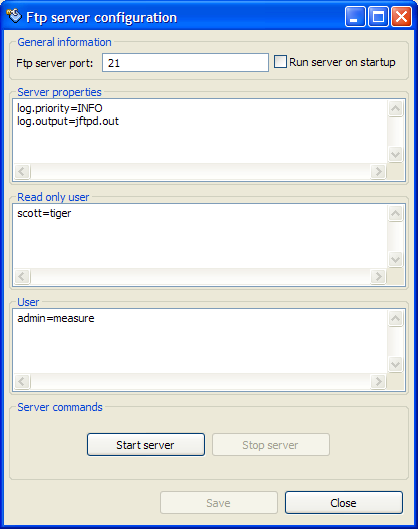
\includegraphics[width=0.6\linewidth]{figures/gui/03.png}
\end{center}
\caption{Okno konfiguracji serwera FTP}\label{rys:ftpwindow}
\end{figure}
Pole tekstowe ,,Server properties'' służy do ustawiania specyficznych właściwości serwera.
Wpisuje się tutaj pary klucz--wartość. W chwili obecnej dostępne są dwa klucze:
\begin{itemize}
\item log.prority -- określa priorytet logowanych operacji dla serwera FTP. Dostępne są następujące wartości:
\begin{itemize}
\item NONE -- powoduje wyłączenie logowania,
\item INFO -- loguje wszystkie dostępne informacje,
\item DEBUG -- loguje błędy i informacje przydatne w procesie debugowania,
\item ERROR -- loguje tylko błędy.
\end{itemize}
Informacje te są zapisywane w pliku wskazywanym przez klucz ,,log.output''.
\item log.output -- wskazuje położenie pliku z logami.
\end{itemize}
Serwer ftp jak i cała aplikacja używa do logowania operacji biblioteki Log4J~\cite{Log4J1}.

Pole tekstowe ,,Read only user'' umożliwia podanie użytkowników z prawami tylko do odczytu z serwera FTP.
W polu tym w każdej linii umieszcza się pary klucz--wartość, gdzie klucz odpowiada loginowi użytkownika,
a wartość to hasło. 

Pole tekstowe ,,User'' umożliwia podanie użytkowników z pełnymi prawami do serwera FTP. Tacy użytkownicy
mogą dodawać, modyfikować i usuwać pliki dostępne na serwerze ftp benchmarku.

\section{Server RMI}\label{sect:rmiserver}
Do komunikacji pomiędzy serwerem, a klientami RTE aplikacja wykorzystuje serwer
RMI~\cite{RMI1}. Można go skonfigurować wybierając z menu ,,Configuration'' opcję ,,RMI server''. 
Wybranie tej opcji powoduje wyświetlenie okienka widocznego na rys.~\ref{rys:rmiwindow}.
\begin{figure}[h]
\begin{center}
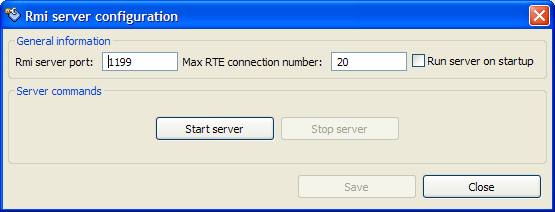
\includegraphics[width=0.70\linewidth]{figures/gui/04.png}
\end{center}
\caption{Okno konfiguracji serwera RMI}\label{rys:rmiwindow}
\end{figure}
Jak widać, w tym miejscu można określić: numer portu na którym ma nasłuchiwać serwer,
maksymalną liczbę klientów RTE, którzy mogą podłączyć się do serwera, czy serwer ma być
uruchamiany wraz z uruchomieniem aplikacji.

\section{Projekt testu}
Aplikacja GUI serwera benchmarku umożliwia tworzenie projektów testów,
które chcemy przeprowadzić. W tym celu należy z menu ,,File'' wybrać opcję ,,Create test...''.
W wyświetlonym kreatorze istnieje możliwość utworzenia pustego projektu, skopiowania modeli
z jednego z istniejących projektów, lub szablonów (zob. rys.~\ref{rys:createproject}).
\begin{figure}[h]
\begin{center}
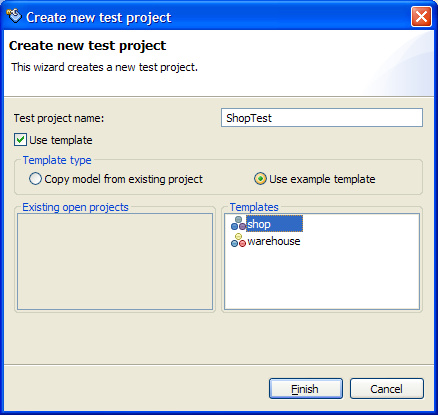
\includegraphics[width=0.5\linewidth]{figures/gui/07.png}
\end{center}
\caption{Kreator projektu testu}\label{rys:createproject}
\end{figure}
Po wybraniu przycisku ,,Finish'' zostanie utworzony projekt testu. Struktura typowego projektu 
została przedstawiona na rys. \ref{rys:testprojectstr}.
\begin{figure}[h]
\begin{center}
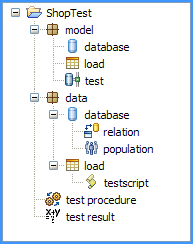
\includegraphics[width=0.3\linewidth]{figures/gui/10.png}
\end{center}
\caption{Struktura projektu testu}\label{rys:testprojectstr}
\end{figure}
Została ona zorganizowana w drzewo dzielące ją na kilka kategorii:
,,model'', ,,data'', ,,test procedure'', ,,test result''. Praca z testem powinna przebiegać
zgodnie z zasadą przechodzenia od liści drzewa usytuowanych najwyżej, do tych usytuowanych najniżej.

Gałąź ,,model'' zawiera modele dostępne dla projektu testu -- są to modele opisane już powyżej, 
a reprezentowane przez liście drzewa: ,,database'', ,,load'' oraz ,,test''.

Gałąź ,,data'' zawiera w sobie wszystkie operacje związane z generowaniem i przygotowywaniem danych niezbędnych
do przeprowadzenia testu. Gałąź ta dzieli się na dwie podgałęzie: ,,database'' -- grupującą operacje
związane z bazą danych, oraz ,,load''-- związaną z generowaniem danych symulujących obciążenie.
W gałęzi ,,database'' dostępne są dwa kreatory: pierwszy do tworzenia bądź usuwania relacji z bazy danych -- ,,relation'',
drugi do generowania populacji -- ,,population''. W gałęzi ,,load'' znajduje się tylko jeden liść -- ,,testscript'', 
reprezentujący kreator tworzenia skryptów testowych. 

Liść ,,test procedure'' reprezentuje kreator przeprowadzania procedury testu.

Liść ,,test result'' zawiera generator raportów i histogramów z wyników przeprowadzonej procedury testu.

\section{Tworzenie modeli}
Aplikacja graficzna serwera benchmarku umożliwia tworzenie modeli bazy danych, obciążenia oraz testu (zob.~rozdz.\ref{rodz:over}). 
Modele te można wpisać posługując się formatem XML, bądź skorzystać z dostępnych formularzy. W załączniku do niniejszej pracy zostały
umieszczone opisy struktury dokumentów xml poszczególnych modeli w postaci XmlSchema~\cite{XmlSchema1}.

\subsection{Model bazy danych}
Model bazy danych można edytować posługując się edytorem dostępnym po wybraniu z
drzewa struktury testu ścieżki ,,model -$>$ database''. W wyniku tej operacji w
głównej części okna aplikacji zostanie wyświetlony edytor modelu bazy danych (zob. rys.~\ref{rys:databaseedytor}).
\begin{figure}[h]
\begin{center}
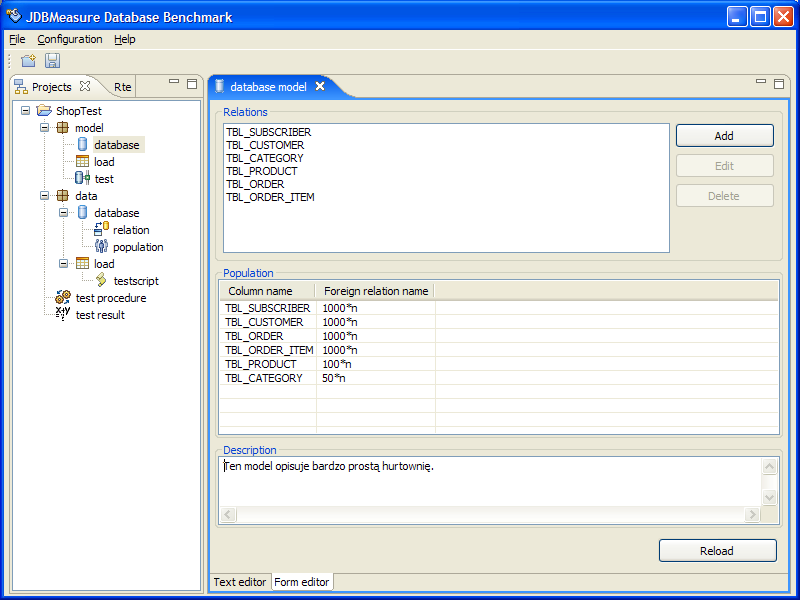
\includegraphics[width=0.9\linewidth]{figures/gui/12.png}
\end{center}
\caption{Edytor modelu bazy danych}\label{rys:databaseedytor}
\end{figure}
W dolnej części edytora znajdują się zakładki umożliwiające przełączanie
pomiędzy edytorem tekstowym, a edytorem opartym o formularze i okna dialogowe.
Edytor tekstowy umożliwia bezpośrednią modyfikację dokumentu xml reprezentującego model bazy danych.
,,Form edytor'' dostarcza natomiast metody modyfikacji dokumentu przy pomocy okien i formularzy.

Sekcja ,,Relations'' edytora umożliwia modyfikację relacji modelu bazy danych. Dostępna jest tutaj lista zdefiniowanych 
relacji. Każdą relację można wyedytować, czy usunąć służą do tego odpowiednio przyciski ,,Edit'' oraz ,,Delete''.
Można również dodać nową relację -- w tym celu należy posłużyć się przyciskiem ,,Add''. 

Sekcja ,,Population'' służy do określenia dla każdej zdefiniowanej relacji, liczby generowanych, w procesie
tworzenia populacji -- rekordów. Można tutaj podać wartość stałą, lub wyrażenie względem parametru skalującego n.

Ostatnią sekcją jest tutaj ,,Description'' -- umożliwia ona podanie opisu tekstowego tworzonego modelu bazy danych.

\subsection{Model obciążenia}
Model obciążenia można edytować posługując się edytorem dostępnym po wybraniu z
drzewa struktury testu ścieżki ,,model -$>$ load''. W wyniku tej operacji w
głównej części okna aplikacji zostanie wyświetlony edytor modelu obciążenia (zob. rys.~\ref{rys:loadedytor}).
\begin{figure}[h]
\begin{center}
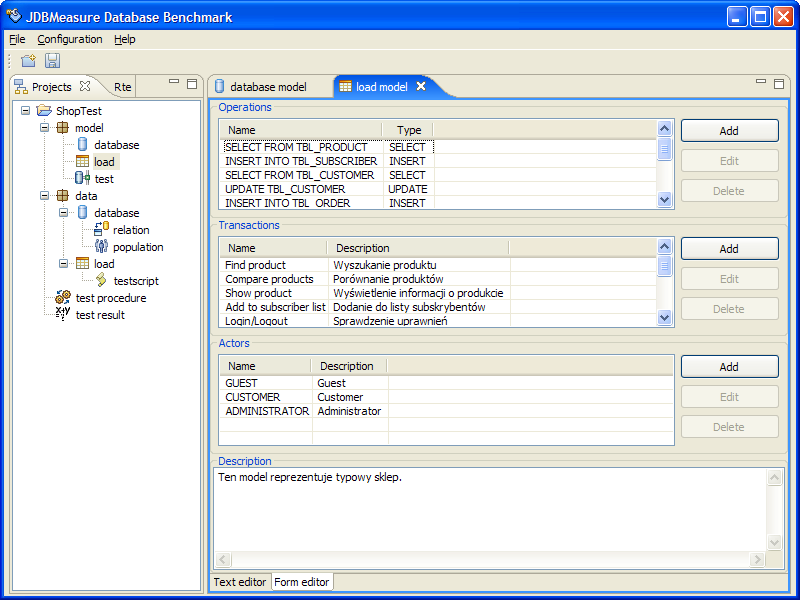
\includegraphics[width=0.9\linewidth]{figures/gui/14.png}
\end{center}
\caption{Edytor modelu obciążenia}\label{rys:loadedytor}
\end{figure}
W dolnej części edytora znajdują się zakładki umożliwiające przełączanie
pomiędzy edytorem tekstowym, a edytorem opartym o formularze i okna dialogowe.
Edytor tekstowy umożliwia bezpośrednią modyfikację dokumentu xml reprezentującego model obciążenia.
,,Form edytor'' dostarcza natomiast metody modyfikacji dokumentu przy pomocy okien i formularzy.

Sekcja ,,Operations'' służy do dodawania i modyfikacji operacji zdefiniowanych w modelu obciążenia.
W tym celu należy posłużyć się przyciskami ,,Add'', ,,Edit'' oraz ,,Delete''.
W sekcji tej znajduje się także lista istniejących w modelu operacji.

Sekcja ,,Transaction'' zawiera listę zdefiniowanych w modelu transakcji. Lista ta może być modyfikowana
za pomocą znajdujących się na prawo od niej przycisków  ,,Add'', ,,Edit'' oraz ,,Delete''.

Sekcja ,,Actors'' jest przeznaczona do edycji listy zdefiniowanych w modelu aktorów. W tym celu należy posłużyć się przyciskami
,,Add'', ,,Edit'' oraz ,,Delete''.

W dolnej części edytora znajduje się sekcja ,,Description'' umożliwiająca wprowadzenie opisu tekstowego dla modelu obciążenia.

\subsection{Model testu}
Model testu można edytować posługując się edytorem dostępnym po wybraniu z
drzewa struktury testu ścieżki ,,model -$>$ test''. W wyniku tej operacji w
głównej części okna aplikacji zostanie wyświetlony edytor modelu test (zob. rys.~\ref{rys:testedytor}).
\begin{figure}[h]
\begin{center}
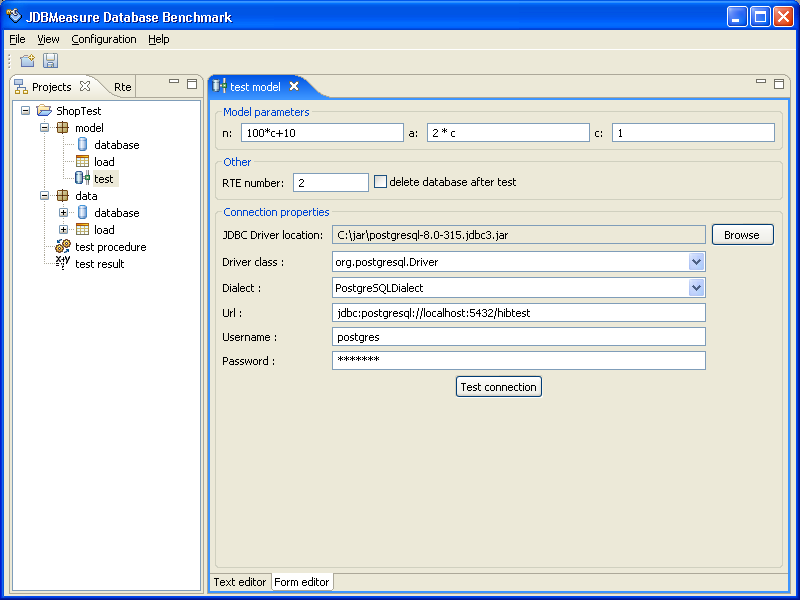
\includegraphics[width=0.9\linewidth]{figures/gui/16.png}
\end{center}
\caption{Edytor modelu testu}\label{rys:testedytor}
\end{figure}
W dolnej części edytora znajdują się zakładki umożliwiające przełączanie
pomiędzy edytorem tekstowym, a edytorem opartym o formularze i okna dialogowe.
Edytor tekstowy umożliwia bezpośrednią modyfikację dokumentu xml reprezentującego model testu.
,,Form edytor'' dostarcza natomiast metody modyfikacji dokumentu przy pomocy okien i formularzy.
Edytor ten umożliwia zdefiniowanie modelu testu, ułatwia przy tym określenie sterownika JDBC,
a także umożliwia przetestowanie połączenia z bazą danych.

Sekcja ,,Model parameters'' umożliwia określenie wartości parametrów skalujących:
\begin{itemize}
\item ,,n'' -- jest parametrem skalującym wykorzystywanym w modelu bazy danych, do określenia liczby 
generowanych rekordów dla poszczególnych relacji, w procesie generowania populacji,
\item ,,a'' -- jest parametrem skalującym wykorzystywanym w modelu obciążenia, do definiowania minimalnej 
i~maksymalnej liczby aktorów danego typu,
\item ,,c'' -- jest parametrem służącym do powiązania parametrów ,,n'' i ,,a''.
\end{itemize}
Więcej informacji na temat parametrów skalujących znajduje się w podpunkcie~\ref{sect:testmodel}.

Sekcja ,,Other'' zawiera opcje konfiguracyjne modelu testu nie sklasyfikowane nigdzie indziej. Można
tutaj określić liczbę RTE biorących udział w teście, jak i to czy baza danych ma być usunięta po zakończeniu testu.
Warto w tym miejscu zauważyć, iż zwiększenie liczby RTE nie powoduje zwiększenia obciążenia, gdyż obciążenie zdefiniowane
w modelu obciążenia jest dzielone na wszystkie RTE biorące udział w teście. Tak więc zwiększając liczbę RTE zmniejszamy
porcję generowanego obciążenia przez pojedyncze RTE. Dla bazy danych rośnie natomiast liczba potencjalnych konfliktów
przydziału zasobów, wynikających z wielodostępu.

Sekcja ,,Connection properties'' zawiera właściwości połączenia do bazy danych. ,,JDBC Driver location'' służy do wskazania
sterownika JDBC, który ma zostać użyty w teście. W celu zmiany wartości tej właściwości należy wybrać przycisk ,,Browse''.
Po dokonaniu tej operacji zostanie wyświetlone okienko, umożliwiające wskazanie lokalizacji sterownika. Warto tutaj zauważyć,
iż sterowniki nie wchodzą bezpośrednio w skład benchmarku. Należy zatem pobrać niezbędny sterownik JDBC ze strony producenta 
testowanego SZBD lub z innej lokalizacji. Lista rozwijana ,,Driver class'' służy do wyboru jednej ze znalezionych w bibliotece 
sterownika JDBC klasy sterownika. Lista rozwijana ,,Dialect'' umożliwia wybór dialektu testowanej bazy danych. To od wybranego dialektu
zależy sposób generowania skryptów tworzących i usuwających bazę danych, a także sposób obsługi obiektów LOB. Kolejną właściwością
jest tutaj ,,Url''. Jest to łańcuch znakowy umożliwiający sterownikowi JDBC zlokalizowanie bazy danych. Dokładna struktura
tego łańcucha zależy od typu bazy danych i od danego sterownika. Dlatego bliższych informacji na ten temat należy szukać w dokumentacji 
używanego sterownika JDBC. Ostatnimi parametrami sekcji są ,,Username'' i ,,Password''. Służą one do uwierzytelniania i 
autoryzacji dostępu do bazy danych.

\begin{figure}[!h]
\begin{center}
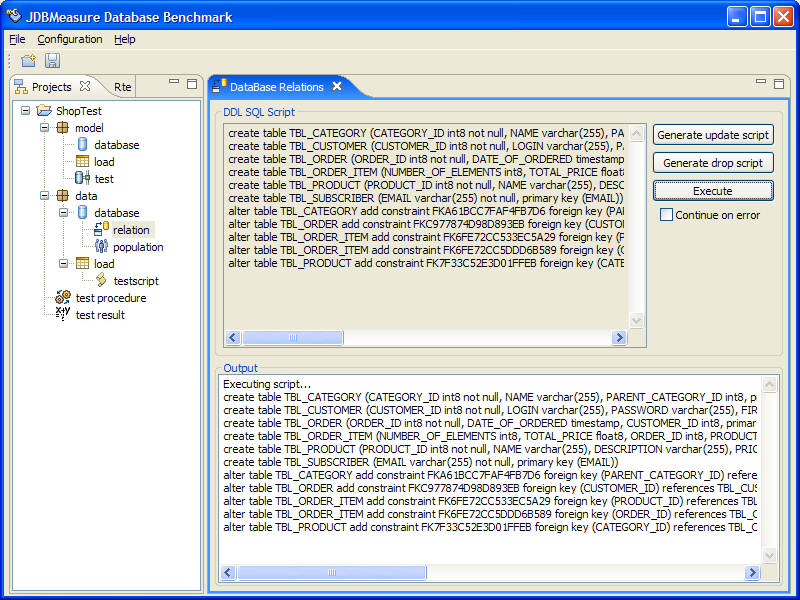
\includegraphics[width=0.9\linewidth]{figures/gui/18.png}
\end{center}
\caption{Edytor relacji}\label{rys:relationsedytor}
\end{figure}

\section{Generowanie danych}
Kolejnym etapem pracy z benchmarkiem -- po zdefiniowaniu modeli, jest przygotowanie
danych potrzebnych w procedurze testu. Dane te można przygotować przy pomocy
edytorów/kreatorów dostępnych w gałęzi data drzewa struktury projektu testu.
\subsection{Tworzenie/usuwanie relacji}
W celu stworzenia na podstawie modelu bazy danych relacji w fizycznej bazie danych
należy wybrać liść ,,data-$>$database-$>$relation''. W wyniku tej operacji zostanie
wyświetlony edytor relacji (zob. rys.~\ref{rys:relationsedytor}).
Edytor ten umożliwia wygenerowanie, dla konkretnego określonego w modelu testu -- DBMS,
skryptów języka SQL, tworzących lub usuwających relacje z bazy danych, a także ich wykonanie.

W celu stworzenia struktury bazy danych należy posłużyć się przyciskiem ,,Generate update script'',
a następnie ,,Execute''. Przycisk ,,Generate update script'' służy do wygenerowania na 
podstawie modelu bazy danych i~modelu testu skryptów tworzących relacje i~powiązania między nimi.

Aby usunąć istniejące relacje, należy wygenerować przyciskiem ,,Generate drop script''
skrypt usuwający relacje, a następnie wykonać go przyciskiem ,,Execute''.

W sekcji ,,DDL SQL Script'' znajduje się pole tekstowe z podglądem wygenerowanych skryptów,
sekcja ,,Output'' zawiera pole tekstowe z komunikatami dotyczącymi wykonywania skryptów.

\subsection{Tworzenie populacji}
Kolejnym edytorem jest tzw. ,,Generator populacji''(zob. rys.~\ref{rys:populationgenerator}). 
Generator ten służy do wygenerowania na podstawie modelu bazy danych, modelu obciążenia 
oraz modelu testu, populacji dla bazy danych. Generator dostępny jest poprzez 
zaznaczenie w drzewie opcji ,,data-$>$database-$>$population''.
\begin{figure}[h]
\begin{center}
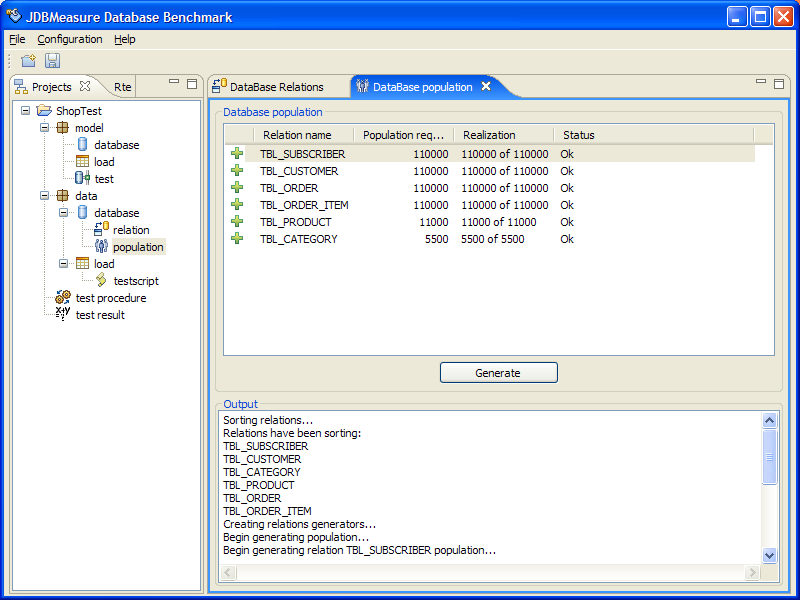
\includegraphics[width=0.9\linewidth]{figures/gui/21.png}
\end{center}
\caption{Generator populacji}\label{rys:populationgenerator}
\end{figure}

\subsection{Przygotowanie skryptów testowych}
Ostatnim narzędziem służącym do przygotowania danych, jest kreator skryptów testowych (zob. rys.~\ref{rys:testscriptscreator}).
W celu wyświetlenia kreatora należy zaznaczyć w drzewie struktury opcję ,,data-$>$load-$>$testscript''
Kreator ten na podstawie wszystkich 3 modeli i zawartości populacji bazy danych
przygotowuje zestaw skryptów testowych. Liczba wygenerowanych skryptów jest zgodna z liczbą RTE wymaganych
do przeprowadzenia procedury testu. Warto zauważyć, że operacja ta nie wymaga 
podłączania RTE do serwera, dzięki temu następuje minimalizacja czasu, w którym 
należy zestawić infrastrukturę testu -- tzn. podłączyć wszystkie wymagane RTE do serwera.
\begin{figure}[h]
\begin{center}
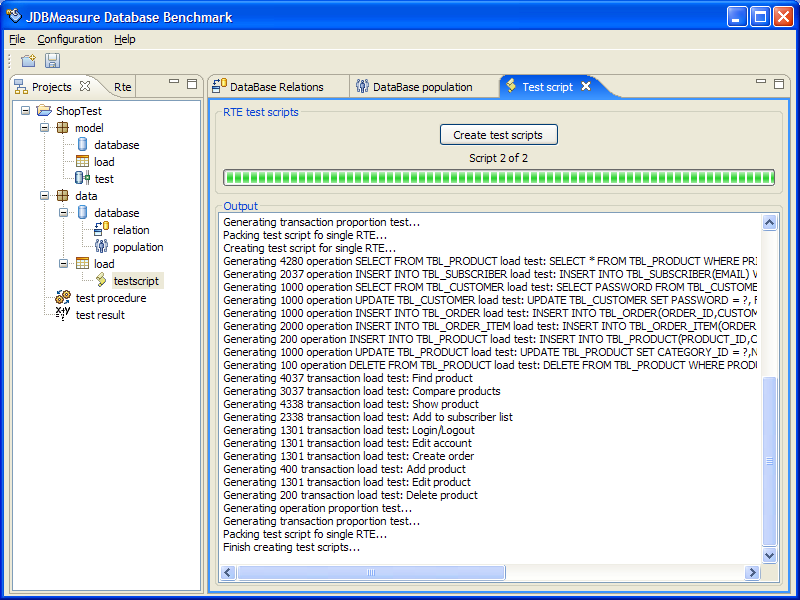
\includegraphics[width=0.9\linewidth]{figures/gui/23.png}
\end{center}
\caption{Kreator skryptów testowych}\label{rys:testscriptscreator}
\end{figure}

\begin{figure}[!h]
\begin{center}
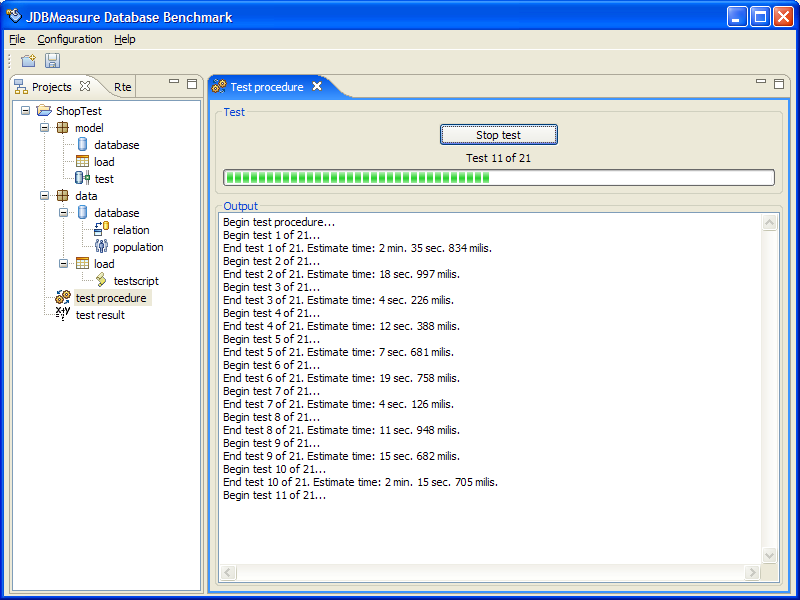
\includegraphics[width=0.9\linewidth]{figures/gui/28.png}
\end{center}
\caption{Przeprowadzanie procedury testu}\label{rys:testprocedure}
\end{figure}

\section{Przeprowadzanie procedury testu}
Przed rozpoczęciem procedury testu należy uruchomić serwer RMI (zob.~\ref{sect:rmiserver}),
a także uruchomić wymaganą liczbę klientów RTE, tak jak omówiono to w rozdz.~\ref{sect:infra}. 
Z przeprowadzaniem procedury testu związany jest widok dostępny po wybraniu z drzewa struktury 
opcji ,,test procedure'' (zob.~rys.~\ref{rys:testprocedure}).

\section{Analiza wyników}
Jeżeli procedura testu zakończyła się powodzeniem można przystąpić do analizy wyników
testów. W tym celu należy przejść do ,,edytora wyników testu'' dostępnego po wybraniu z
drzewa struktury opcji ,,test result''. W edytorze testu dostępne są trzy zakładki
omówione poniżej.

\subsection{Raport tekstowy}
Raport tekstowy jest elementem pierwszej zakładki ,,edytora wyników testu''(zob. rys.~\ref{rys:textraport}). Raport ten został
omówiony szczegółowo w punkcie \ref{sect:textraport}. W załączniku dostępny
jest wydruk przykładowego raportu.
\begin{figure}[h]
\begin{center}
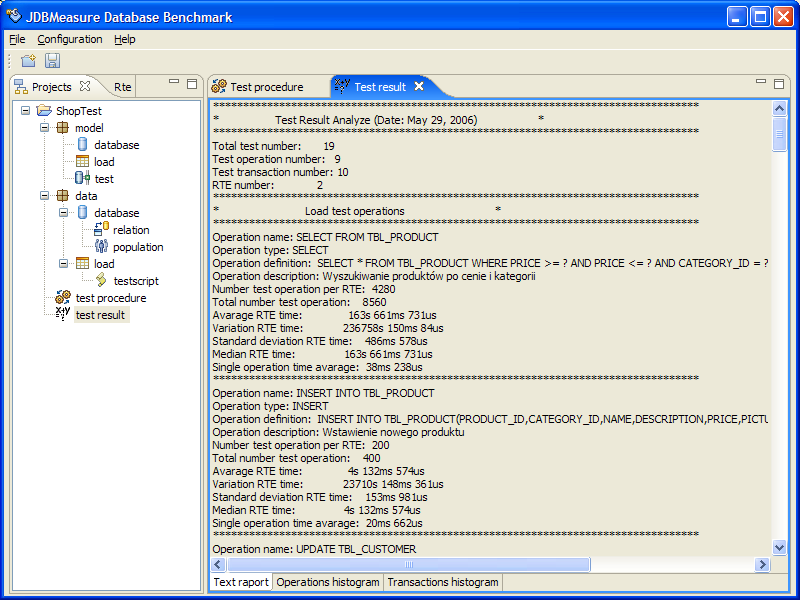
\includegraphics[width=0.9\linewidth]{figures/gui/30.png}
\end{center}
\caption{Raport tekstowy}\label{rys:textraport}
\end{figure}

\subsection{Wykresy}
Pozostałe dwie zakładki ,,edytora wyników testu'' stanowią wykresy histogramów
dla operacji(zob. rys.~\ref{rys:histoper}) i transakcji(zob. rys.~\ref{rys:histtrans}).
Histogramy te obrazują rozkład odpowiedzi dla operacji/transakcji. Możliwe jest określenie
liczby przedziałów histogramów. Wykresy udostępniają funkcje umożliwiające skalowanie,
a także wydruk. Podczas tworzenia histogramów wykorzystano darmową bibliotekę JFreeChart~\cite{JFreeChart1}.
W górnej części zakładki ,,Operations histogram'' znajduje się rozwijana lista, umożliwiająca wybranie interesującej operacji,
na prawo od niej w polu ,,Partitions number'' można określić liczbę przedziałów dla histogramu. Odświeżenie wykresu 
następuje po wyborze przycisku ,,Refresh''. Klikając prawym przyciskiem myszy na obszarze wykresu uzyskuje się dostęp
do menu kontekstowego z opcjami konfiguracyjnymi, a także możliwością wydrukowania wykresu. Przytrzymanie lewego przycisku myszy 
na obszarze wykresu, a następnie przeciągnięcie kursora i puszczenie przycisku, powoduje powiększenie prostokątnego obszaru,
o przekątnej pomiędzy punktem przytrzymania, a puszczenia. Podobną funkcjonalność posiada zakładka ,,Transactions histogram''. 

\begin{figure}[!h]
\begin{center}
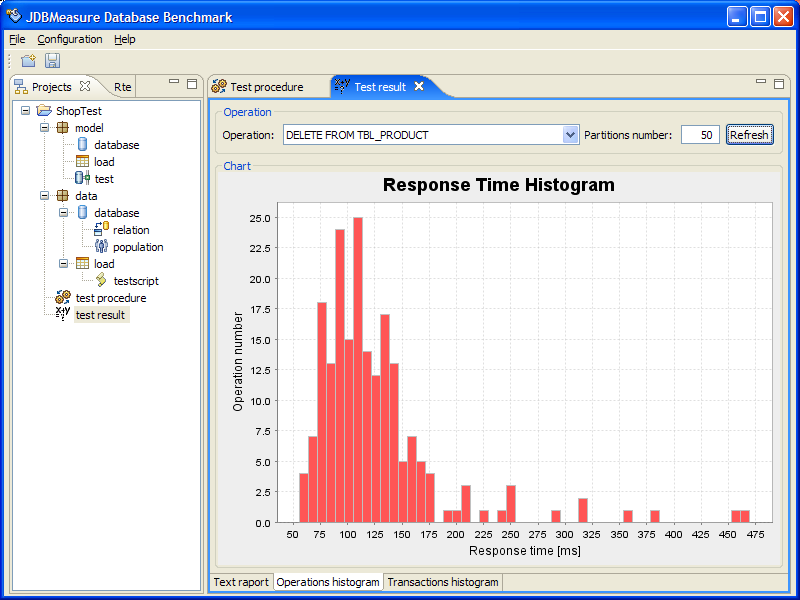
\includegraphics[width=0.9\linewidth]{figures/gui/31.png}
\end{center}
\caption{Histogram czasu wykonania operacji}\label{rys:histoper}
\end{figure}

\begin{figure}[!h]
\begin{center}
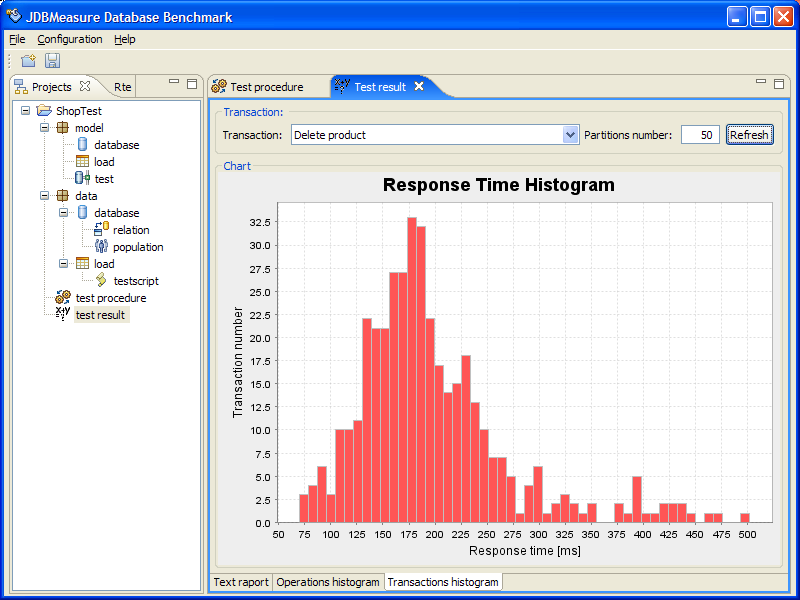
\includegraphics[width=0.9\linewidth]{figures/gui/32.png}
\end{center}
\caption{Histogram czasu wykonania transakcji}\label{rys:histtrans}
\end{figure}

\section{Podsumowanie}
Interfejs graficzny aplikacji serwera benchmarku umożliwia wykonanie
wszystkich niezbędnych operacji, z jakimi użytkownik może mieć do czynienia,
podczas pracy z benchmarkiem. Udostępnia mechanizmy umożliwiające kopiowanie modeli z istniejących projektów,
jak i użycie szablonów sklepu lub hurtowni. Ponadto dzięki poczynionym staraniom automatyzuje
szereg żmudnych i czasochłonnych działań. Dzięki zastosowanym technologiom -- Eclipse RCP \cite{RCP1}, możliwe jest łatwe
rozszerzanie jej o nowe funkcjonalności takie jak:
\begin{enumerate}
\item Edytor XML z podpowiadaniem składni, ułatwiający edycję modeli.
\item Edytory graficzne oparte o biblioteki GEF~\cite{GEF1}, EMF~\cite{EMF1} lub GMF~\cite{GMF1}. Takie edytory 
umożliwiły by wizualne tworzenie modeli tak jak zostało to zilustrowane na rys.~\ref{rys:database-model} 
oraz rys.~\ref{rys:load-model}.
\end{enumerate}

